% ----------------------------------------------------------
% Desenvolvimento do Projeto
% ----------------------------------------------------------
\chapter{Desenvolvimento do Projeto}

Este capítulo descreve o que o sistema faz, como ele foi organizado e quais tecnologias, testes, regras de segurança, banco de dados e prazos fazem parte do projeto.

\section{Escopo do Projeto}

O escopo compreende o desenvolvimento de uma SPA (\textit{Single Page Application}) integrada a uma API RESTful. Nesta seção estão as regras de negócio, os requisitos funcionais e os requisitos não funcionais.

\subsection{Regras de Negócio (RN)}

As regras de negócio dizem como o sistema deve se comportar em cada situação do dia a dia do criador de conteúdo. As seis primeiras vêm do levantamento inicial do projeto.

\begin{itemize}
    \item \textbf{RN01 -- Fluxo de Aprovação:} uma ``Ideia'' só pode ser convertida em ``Projeto de Conteúdo'' depois que o público-alvo e o objetivo pedagógico forem preenchidos. O sistema recusa a conversão com campos vazios ou curtos demais: o título e o público-alvo precisam ter pelo menos 3 caracteres, e o objetivo, pelo menos 10.

    \item \textbf{RN02 -- Versionamento de Roteiro:} o roteiro mantém um histórico de versões. Cada versão salva é uma cópia completa do texto e pode ser restaurada.

    \item \textbf{RN03 -- Consistência de Grade:} um curso não pode ser publicado se não tiver módulos, se tiver módulos sem aulas, se tiver aulas sem material ou se tiver aulas com link inválido. Uma aula está sem material quando não tem nenhum material ligado a ela e nenhum link de conteúdo. Enquanto houver problemas, a publicação fica bloqueada.

    \item \textbf{RN04 -- Gestão de Armazenamento:} uma rotina diária move para o Amazon S3 Glacier (classe \textit{Instant Retrieval}) os materiais de cursos publicados há mais de 30 dias. Isso reduz o custo de armazenamento sem impedir o \textit{download}.

    \item \textbf{RN05 -- Unicidade de Identificação:} cada conteúdo (ideia ou projeto, roteiro, material, curso, módulo e aula) recebe um UUID (\textit{Universally Unique Identifier}) na criação. A API devolve esse identificador, que permite a \textit{scripts} e ferramentas externas acompanhar o mesmo conteúdo da ideia até a publicação.

    \item \textbf{RN06 -- Regra de Status:} um curso só é publicado se os links das aulas forem válidos. A verificação de publicação valida cada link por expressão regular (\textit{Regex}). São aceitos links do YouTube, do Vimeo e links HTTPS de plataformas de ensino (LMS) cadastradas na configuração do sistema, como Moodle e Google Classroom.
\end{itemize}

\textbf{Detalhamento da RN06.} As expressões regulares usadas na validação são as seguintes:

\begin{small}
\begin{verbatim}
[PREENCHER: expressão regular do YouTube, copiada do código]
[PREENCHER: expressão regular do Vimeo, copiada do código]
[PREENCHER: expressão regular dos links de LMS cadastrados]
\end{verbatim}
\end{small}

Exemplos de links \textbf{válidos}: [PREENCHER: um link do YouTube, um do Vimeo e um de LMS cadastrado]. Exemplos de links \textbf{inválidos}: [PREENCHER: um link de plataforma não cadastrada e um link sem \textit{https}].

Durante o desenvolvimento, a equipe definiu outras regras que o sistema também aplica:

\begin{itemize}
    \item \textbf{Equipe:} toda equipe tem pelo menos um Administrador. O último Administrador não pode ser removido, rebaixado nem sair sem passar a administração para outra pessoa.
    \item \textbf{Votos:} cada membro vota uma única vez em cada ideia. Um segundo clique retira o voto.
    \item \textbf{Revisão:} pedir ajustes exige um comentário. Ideias que ainda não viraram projeto não recebem revisão.
    \item \textbf{Convites:} o convite vale 7 dias e é pessoal. Só a conta com o mesmo e-mail pode aceitá-lo.
    \item \textbf{Códigos por e-mail:} os códigos valem 10 minutos e aceitam até 5 tentativas.
    \item \textbf{Resumo automático:} o resumo exige um roteiro com pelo menos 100 palavras.
    \item \textbf{Materiais:} os arquivos podem ter até 20 MB e precisam ser de um dos tipos permitidos.
\end{itemize}

\subsection{Requisitos Funcionais (RF)}

Os requisitos funcionais dizem o que o sistema faz. Eles estão agrupados por módulo, para facilitar a leitura.

\textbf{Módulo de Autenticação e Perfil}

\begin{itemize}
    \item \textbf{RF01:} cadastrar usuários em duas etapas. O usuário informa nome e e-mail, recebe um código de 6 dígitos por e-mail e, com ele, define a senha. O sistema também permite recuperar a senha por código, trocar o e-mail e excluir a conta.
    \item \textbf{RF02:} controlar o acesso por funções (RBAC) em cada equipe: Administrador, Criador e Revisor. A mesma pessoa pode ter papéis diferentes em equipes diferentes. A Tabela~\ref{tab:permissoes} mostra o que cada papel pode fazer.
\end{itemize}

\begin{table}[H]
\centering
\caption{Permissões por papel na equipe}
\label{tab:permissoes}
\small
\begin{tabular}{|p{8cm}|c|c|c|}
\hline
\textbf{Ação} & \textbf{Administrador} & \textbf{Criador} & \textbf{Revisor} \\
\hline
Ver quadro, ideias, roteiros, materiais e cursos & Sim & Sim & Sim \\
\hline
Votar em ideias e marcar tarefas como feitas & Sim & Sim & Sim \\
\hline
Criar ideias, converter em projeto, mover e excluir \textit{cards} & Sim & Sim & Não \\
\hline
Criar, editar e atribuir tarefas & Sim & Sim & Não \\
\hline
Escrever e versionar roteiros, gerar resumo, enviar materiais & Sim & Sim & Não \\
\hline
Criar, editar, publicar e exportar cursos & Sim & Sim & Não \\
\hline
Registrar revisão (aprovar ou pedir ajustes) & Sim & Não & Sim \\
\hline
Gerenciar colunas e etiquetas & Sim & Não & Não \\
\hline
Convidar, remover membros e mudar papéis & Sim & Não & Não \\
\hline
Renomear e excluir a equipe & Sim & Não & Não \\
\hline
Sair da equipe & Sim & Sim & Sim \\
\hline
\end{tabular}
\end{table}

\textbf{Módulo de Gestão de Ideias (Inbox)}

\begin{itemize}
    \item \textbf{RF03:} permitir a criação de \textit{cards} de ideias com \textit{tags} coloridas. Cada equipe tem a sua lista de etiquetas, que começa com Tutorial, Podcast, Curso, Roteiro e Artigo.
    \item \textbf{RF04:} ter um sistema de votação para priorizar as ideias em equipe. O \textit{card} mostra o total de votos, e a Caixa de Entrada pode ser ordenada por votos.
\end{itemize}

\textbf{Módulo de Produção (Workflow)}

\begin{itemize}
    \item \textbf{RF05:} oferecer um quadro \textit{Kanban} com colunas configuráveis por equipe. As colunas padrão são Pesquisa, Roteiro, Gravação e Edição. Cada projeto tem tarefas com responsável e prazo, e o progresso é calculado automaticamente pelas tarefas concluídas.
    \item \textbf{RF06:} permitir o \textit{upload} de materiais de apoio (PDF, Word, PowerPoint, Excel, texto e imagens PNG, JPG, WEBP e GIF) de até 20 MB, ligados ao projeto e guardados no Amazon S3.
    \item \textbf{RF07:} oferecer um editor de texto rico (\textit{Rich Text}), chamado Estúdio de Escrita, para escrever roteiros dentro da plataforma, com histórico de versões.
\end{itemize}

\textbf{Módulo de Automação}

\begin{itemize}
    \item \textbf{RF08:} gerar um resumo do conteúdo do projeto a partir do roteiro. O \textit{back-end} envia o texto do roteiro a um serviço de automação escrito em Python, que devolve o resumo.
    \item \textbf{RF09:} mostrar um painel de alertas com os projetos e as tarefas atrasados ou que vencem nos próximos 3 dias. Todos os dias, às 8h (horário de Brasília), cada pessoa recebe um único e-mail com os prazos vencidos e próximos de todas as suas equipes.
\end{itemize}

\textbf{Módulo de Estruturação Curricular (LMS Ready)}

\begin{itemize}
    \item \textbf{RF10:} permitir a criação de cursos e a organização dos conteúdos em módulos e aulas (vídeo, texto ou questionário).
    \item \textbf{RF11:} exportar a estrutura do curso em JSON ou CSV, para usar em plataformas externas.
\end{itemize}

Além dos requisitos acima, o sistema oferece a revisão de projetos (aprovar ou pedir ajustes), os convites por e-mail para novos membros, a gestão da equipe, a gestão da conta do usuário e o controle dos planos de assinatura, com um plano Gratuito e um teste grátis de 14 dias dos planos pagos.

\subsection{Requisitos Não Funcionais (RNF)}

Os requisitos não funcionais dizem como o sistema funciona: com que segurança, com que velocidade e com que facilidade de manutenção.

\textbf{Segurança e Confiabilidade}

\begin{itemize}
    \item \textbf{RNF01:} as senhas são criptografadas com o algoritmo BCrypt e nunca aparecem nas respostas da API.
    \item \textbf{RNF03:} a autenticação usa \textit{tokens} JWT assinados, válidos por 24 horas e enviados no cabeçalho \textit{Authorization}.
\end{itemize}

\textbf{Performance e Escalabilidade}

\begin{itemize}
    \item \textbf{RNF05:} os e-mails (códigos, convites e alertas) são enviados de forma assíncrona, sem atrasar a resposta da API.
    \item \textbf{RNF06:} o banco de dados está normalizado até a 3ª Forma Normal (3FN), com chaves estrangeiras e regras de exclusão em cascata.
\end{itemize}

\textbf{Infraestrutura e Manutenibilidade}

\begin{itemize}
    \item \textbf{RNF07:} o \textit{back-end} tem testes unitários com JUnit 5 e Mockito, e a cobertura é medida pelo JaCoCo. A meta é acima de 70\%.
    \item \textbf{RNF08:} a documentação da API é gerada automaticamente pelo Swagger (OpenAPI), com o springdoc.
    \item \textbf{RNF09:} o \textit{front-end}, o \textit{back-end} e o serviço de automação em Python rodam em contêineres Docker, com imagens no Amazon ECR, orquestrados pelo Amazon EKS.
    \item \textbf{RNF10:} os \textit{logs} dos contêineres são enviados ao Amazon CloudWatch Logs.
\end{itemize}

\section{Histórias de Usuário}

As histórias de usuário descrevem o que cada tipo de pessoa quer fazer no sistema. Aqui elas são apresentadas, detalhadas em critérios de aceitação que podem ser testados e ligadas aos cenários de teste.

\subsection{Descrição das Histórias de Usuário}

As histórias seguem o formato padrão \textit{``Como [perfil], quero [ação], para [valor]''} e vêm dos requisitos funcionais.

\begin{table}[H]
\centering
\caption{Histórias de Usuário}
\label{tab:historias}
\small
\begin{tabular}{|p{0.9cm}|p{2.2cm}|p{7.2cm}|p{3cm}|}
\hline
\textbf{ID} & \textbf{Perfil} & \textbf{História} & \textbf{Cenários de aceitação} \\
\hline
US01 & Criador & Como criador, quero capturar uma ideia rapidamente com título e descrição, para não perder \textit{insights} durante o processo criativo. & CT01, CT02 \\
\hline
US02 & Criador & Como criador, quero mover um conteúdo entre as etapas do \textit{Kanban}, para acompanhar o progresso da produção. & CT03 \\
\hline
US03 & Criador & Como criador, quero ativar um projeto a partir de uma ideia preenchendo o Público-Alvo e o Objetivo Pedagógico, para estruturar formalmente a produção. & CT04, CT05 \\
\hline
US04 & Criador & Como criador, quero fazer \textit{upload} de arquivos PDF e imagens ligados a um projeto, para centralizar os materiais de apoio. & CT06, CT07 \\
\hline
US05 & Criador & Como criador, quero escrever o roteiro direto na plataforma com um editor de texto rico, para evitar o uso de ferramentas externas. & CT08, CT09 \\
\hline
US06 & Administrador & Como administrador, quero convidar colaboradores com perfis diferentes (Criador/Revisor), para controlar o acesso às funcionalidades. & CT10, CT11, CT12 \\
\hline
US07 & Criador & Como criador, quero organizar conteúdos em Módulos e Aulas dentro de um Curso, para estruturar o currículo pedagógico. & CT13, CT14, CT15 \\
\hline
US08 & Criador & Como criador, quero exportar a estrutura do curso em JSON ou CSV, para integrá-la a plataformas externas de LMS. & CT16, CT17 \\
\hline
\end{tabular}
\end{table}

\subsection{Critérios de Aceitação em Gherkin}

Para que cada critério possa ser testado de forma objetiva, eles foram escritos no formato \textit{Gherkin} (Dado/Quando/Então). Cada cenário recebe um código (CT), usado na tabela de rastreabilidade.

\begin{small}

\textbf{US01: Capturar ideia}

\textbf{CT01: Criar ideia com título.} \textbf{Dado} que sou um criador autenticado e estou na Caixa de Entrada, \textbf{quando} preencho o título e salvo, \textbf{então} um \textit{card} com esse título aparece na Caixa de Entrada.

\textbf{CT02: Título obrigatório.} \textbf{Dado} que estou criando uma ideia, \textbf{quando} tento salvar sem título, \textbf{então} o \textit{card} não é criado e o sistema mostra uma mensagem de erro.

\textbf{US02: Mover conteúdo no Kanban}

\textbf{CT03: Mudar de coluna.} \textbf{Dado} que um projeto está na coluna Pesquisa, \textbf{quando} o movo para a coluna Roteiro, \textbf{então} o projeto aparece na nova coluna e o histórico do \textit{card} registra a coluna, a data e quem fez a mudança.

\textbf{US03: Ativar projeto}

\textbf{CT04: Campos vazios ou curtos (RN01).} \textbf{Dado} que tenho uma ideia, \textbf{quando} tento convertê-la com o público-alvo vazio ou com o objetivo pedagógico de menos de 10 caracteres, \textbf{então} o sistema recusa a conversão e informa o campo com problema.

\textbf{CT05: Conversão válida.} \textbf{Dado} que informei título, público-alvo e objetivo pedagógico válidos e não escolhi coluna, \textbf{quando} confirmo a conversão, \textbf{então} o projeto é criado na primeira coluna do quadro.

\textbf{US04: Enviar materiais}

\textbf{CT06: Envio válido (RF06).} \textbf{Dado} que estou em um projeto, \textbf{quando} envio um arquivo PDF de até 20 MB, \textbf{então} o arquivo aparece na lista de materiais com nome, tipo, tamanho, autor e data.

\textbf{CT07: Arquivo recusado.} \textbf{Dado} que estou em um projeto, \textbf{quando} envio um arquivo de tipo não permitido ou maior que 20 MB, \textbf{então} o envio é recusado e o sistema mostra uma mensagem de erro.

\textbf{US05: Escrever roteiro}

\textbf{CT08: Editor de texto rico (RF07).} \textbf{Dado} que abri o Estúdio de Escrita de um projeto, \textbf{quando} escrevo um roteiro com negrito e lista e salvo, \textbf{então} ao abrir de novo o roteiro mantém a formatação.

\textbf{CT09: Restaurar versão (RN02).} \textbf{Dado} que salvei duas versões do roteiro, \textbf{quando} restauro a primeira, \textbf{então} o texto do editor volta a ser o da primeira versão.

\textbf{US06: Convidar colaboradores}

\textbf{CT10: Convite com papel (RF02).} \textbf{Dado} que sou Administrador, \textbf{quando} convido um e-mail com o papel Revisor, \textbf{então} o convite fica pendente por 7 dias e, ao ser aceito pela conta com esse e-mail, a pessoa entra na equipe como Revisor.

\textbf{CT11: Ação sem permissão.} \textbf{Dado} que sou Revisor, \textbf{quando} tento mover um \textit{card}, \textbf{então} a API responde com o código 403 e a mensagem ``Seu papel na equipe não permite esta ação''.

\textbf{CT12: Último administrador.} \textbf{Dado} que sou o único Administrador da equipe, \textbf{quando} tento sair ou me rebaixar, \textbf{então} o sistema recusa e pede que eu promova outra pessoa antes.

\textbf{US07: Organizar o curso}

\textbf{CT13: Hierarquia do curso (RF10).} \textbf{Dado} que tenho um curso, \textbf{quando} crio um módulo e adiciono aulas a ele, \textbf{então} a hierarquia Curso $\rightarrow$ Módulo $\rightarrow$ Aula é salva e mostrada na ordem criada.

\textbf{CT14: Publicação bloqueada (RN03).} \textbf{Dado} que um curso tem um módulo sem aulas, \textbf{quando} tento publicá-lo, \textbf{então} o sistema lista o problema e a publicação é bloqueada.

\textbf{CT15: Link inválido (RN06).} \textbf{Dado} que um curso tem uma aula com um link que não é do YouTube, do Vimeo nem de um LMS cadastrado, \textbf{quando} tento publicá-lo, \textbf{então} o sistema lista a aula com link inválido e a publicação é bloqueada.

\textbf{US08: Exportar o curso}

\textbf{CT16: Exportar em JSON (RF11).} \textbf{Dado} que tenho um curso estruturado, \textbf{quando} exporto em JSON, \textbf{então} o arquivo traz o curso, os módulos, as aulas e os materiais.

\textbf{CT17: Exportar em CSV (RF11).} \textbf{Dado} que tenho um curso estruturado, \textbf{quando} exporto em CSV, \textbf{então} o arquivo, separado por ponto e vírgula e em UTF-8, traz uma linha para cada aula, com os dados do módulo a que ela pertence.

\end{small}

\subsection{Rastreabilidade entre Histórias de Usuário e Testes}

A Tabela~\ref{tab:rastreabilidade} mostra qual cenário de teste cobre cada história de usuário. O tipo de teste segue a pirâmide descrita na seção de testes.

\begin{table}[H]
\centering
\caption{Rastreabilidade entre Histórias de Usuário (US) e Cenários de Teste (CT)}
\label{tab:rastreabilidade}
\small
\begin{tabular}{|p{1.2cm}|p{2.8cm}|p{2.6cm}|p{3.4cm}|p{2.6cm}|}
\hline
\textbf{US} & \textbf{Requisito ou regra} & \textbf{Cenários} & \textbf{Tipo de teste} & \textbf{Situação} \\
\hline
US01 & RF03 & CT01, CT02 & Unitário e integração & Aprovado \\
\hline
US02 & RF05 & CT03 & Integração & Aprovado \\
\hline
US03 & RN01 & CT04, CT05 & Unitário & Aprovado \\
\hline
US04 & RF06 & CT06, CT07 & Integração & Aprovado \\
\hline
US05 & RF07, RN02 & CT08, CT09 & Unitário e componente (Jest) & Aprovado \\
\hline
US06 & RF02 & CT10, CT11, CT12 & Unitário e integração & Aprovado \\
\hline
US07 & RF10, RN03, RN06 & CT13, CT14, CT15 & Unitário e integração & Aprovado \\
\hline
US08 & RF11 & CT16, CT17 & Integração & Aprovado \\
\hline
\end{tabular}
\end{table}

\section{Arquitetura}

A arquitetura define como as partes do sistema se organizam e conversam entre si.

\subsection{Definições da Arquitetura}

O Creator Workbench adota o padrão \textit{Client-Server} desacoplado (\textit{Decoupled Architecture}). O \textit{front-end} é uma aplicação de página única (SPA), feita em Next.js e publicada como arquivos estáticos. O \textit{back-end} é uma API REST feita em Spring Boot. Os dois são independentes e conversam por HTTP, com dados em JSON, e cada requisição protegida leva o \textit{token} JWT do usuário no cabeçalho \textit{Authorization}.

Essa escolha traz três vantagens: (1) o \textit{front-end} e o \textit{back-end} podem ser publicados e versionados separadamente; (2) a API pode ser testada sozinha, com o Swagger gerado automaticamente; (3) novos clientes, como um aplicativo de celular, podem usar a mesma API sem mudar o servidor.

O \textit{back-end} é dividido em camadas. O \textit{controller} recebe a requisição HTTP. O caso de uso, uma classe para cada ação do sistema, guarda as regras de negócio. O serviço acessa os dados e monta as respostas, e o repositório faz as consultas ao banco. Essa divisão deixa cada regra em um único lugar e facilita os testes. Os dados ficam em um banco MySQL, e a estrutura das tabelas é versionada por migrações Flyway.

Na infraestrutura, o sistema roda na AWS em contêineres Docker orquestrados pelo Amazon EKS (Kubernetes), dentro de uma VPC. São três contêineres: o \textit{front-end} (Nginx servindo os arquivos estáticos do Next.js), o \textit{back-end} (Spring Boot) e o serviço de automação em Python, que gera os resumos. As imagens ficam no Amazon ECR. Um Elastic Load Balancer recebe o acesso dos usuários e o entrega ao \textit{front-end}, que encaminha as chamadas \texttt{/api} para o \textit{back-end}. Os dados ficam no Amazon RDS (MySQL), acessível apenas de dentro da VPC. Os materiais enviados ficam no Amazon S3, e os de cursos publicados há mais de 30 dias passam para o S3 Glacier. Os \textit{logs} dos contêineres vão para o Amazon CloudWatch, e os e-mails do sistema saem por um servidor SMTP.

\subsection{Diagrama da Arquitetura}

O diagrama abaixo mostra as partes do sistema e como elas se comunicam.

\begin{figure}[H]
    \centering
    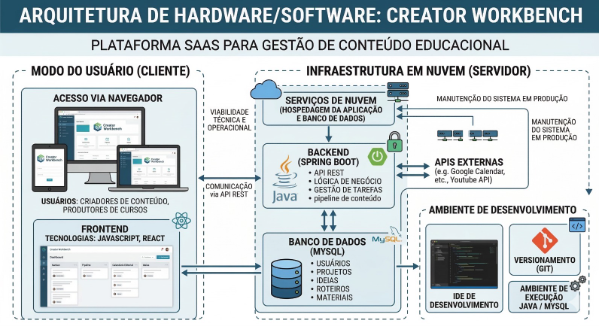
\includegraphics[width=0.85\textwidth]{imagens/diagrama_arq}
    \caption{Diagrama da Arquitetura Client-Server Desacoplado}
    \label{fig:arquitetura}
    \legend{Fonte: Produzido pelos autores.}
\end{figure}

\subsection{Diagrama de Componentes}

O diagrama de componentes mostra as partes internas de cada aplicação e como elas dependem umas das outras (visão \textit{white-box}). A Figura~\ref{fig:componentes} apresenta o \textit{front-end}, o \textit{back-end} e os serviços externos com que eles se comunicam.

No \textit{front-end}, as telas e funcionalidades (autenticação, painel, ideias, quadro Kanban, detalhes do \textit{card}, editor de roteiro, cursos, equipes e configurações do usuário) usam o módulo de estado (\texttt{useAppStore}) e o controle de acesso por papel (\texttt{roles.ts}). O módulo de estado é quem chama a API, por meio do cliente HTTP (\texttt{api.ts}).

No \textit{back-end}, toda requisição passa primeiro pelo módulo de segurança, que valida o \textit{token} com o módulo JWT, e depois chega aos \textit{controllers}. Os \textit{controllers} chamam os casos de uso e serviços de cada módulo de domínio, e estes acessam o banco pela camada de repositório (Spring Data JPA/Hibernate), seguindo as camadas descritas na seção anterior. Alguns módulos falam com serviços de fora da aplicação: o Summary Module chama o serviço Python (\texttt{POST /summarize}), o Material Module guarda os arquivos no Amazon S3 e o Email Module envia os e-mails pelo servidor SMTP. As rotinas agendadas (\textit{Scheduled Jobs}) rodam no próprio Spring Boot: apagam códigos de verificação vencidos, enviam o e-mail diário de prazos e arquivam os materiais antigos. Os três contêineres enviam seus \textit{logs} ao Amazon CloudWatch.

\begin{figure}[p]
    \centering
    \rotatebox{90}{%
    \begin{minipage}{0.95\textheight}
        \centering
        \caption{Diagrama de Componentes (\textit{White-Box}) - Creator Workbench}
        \label{fig:componentes}
        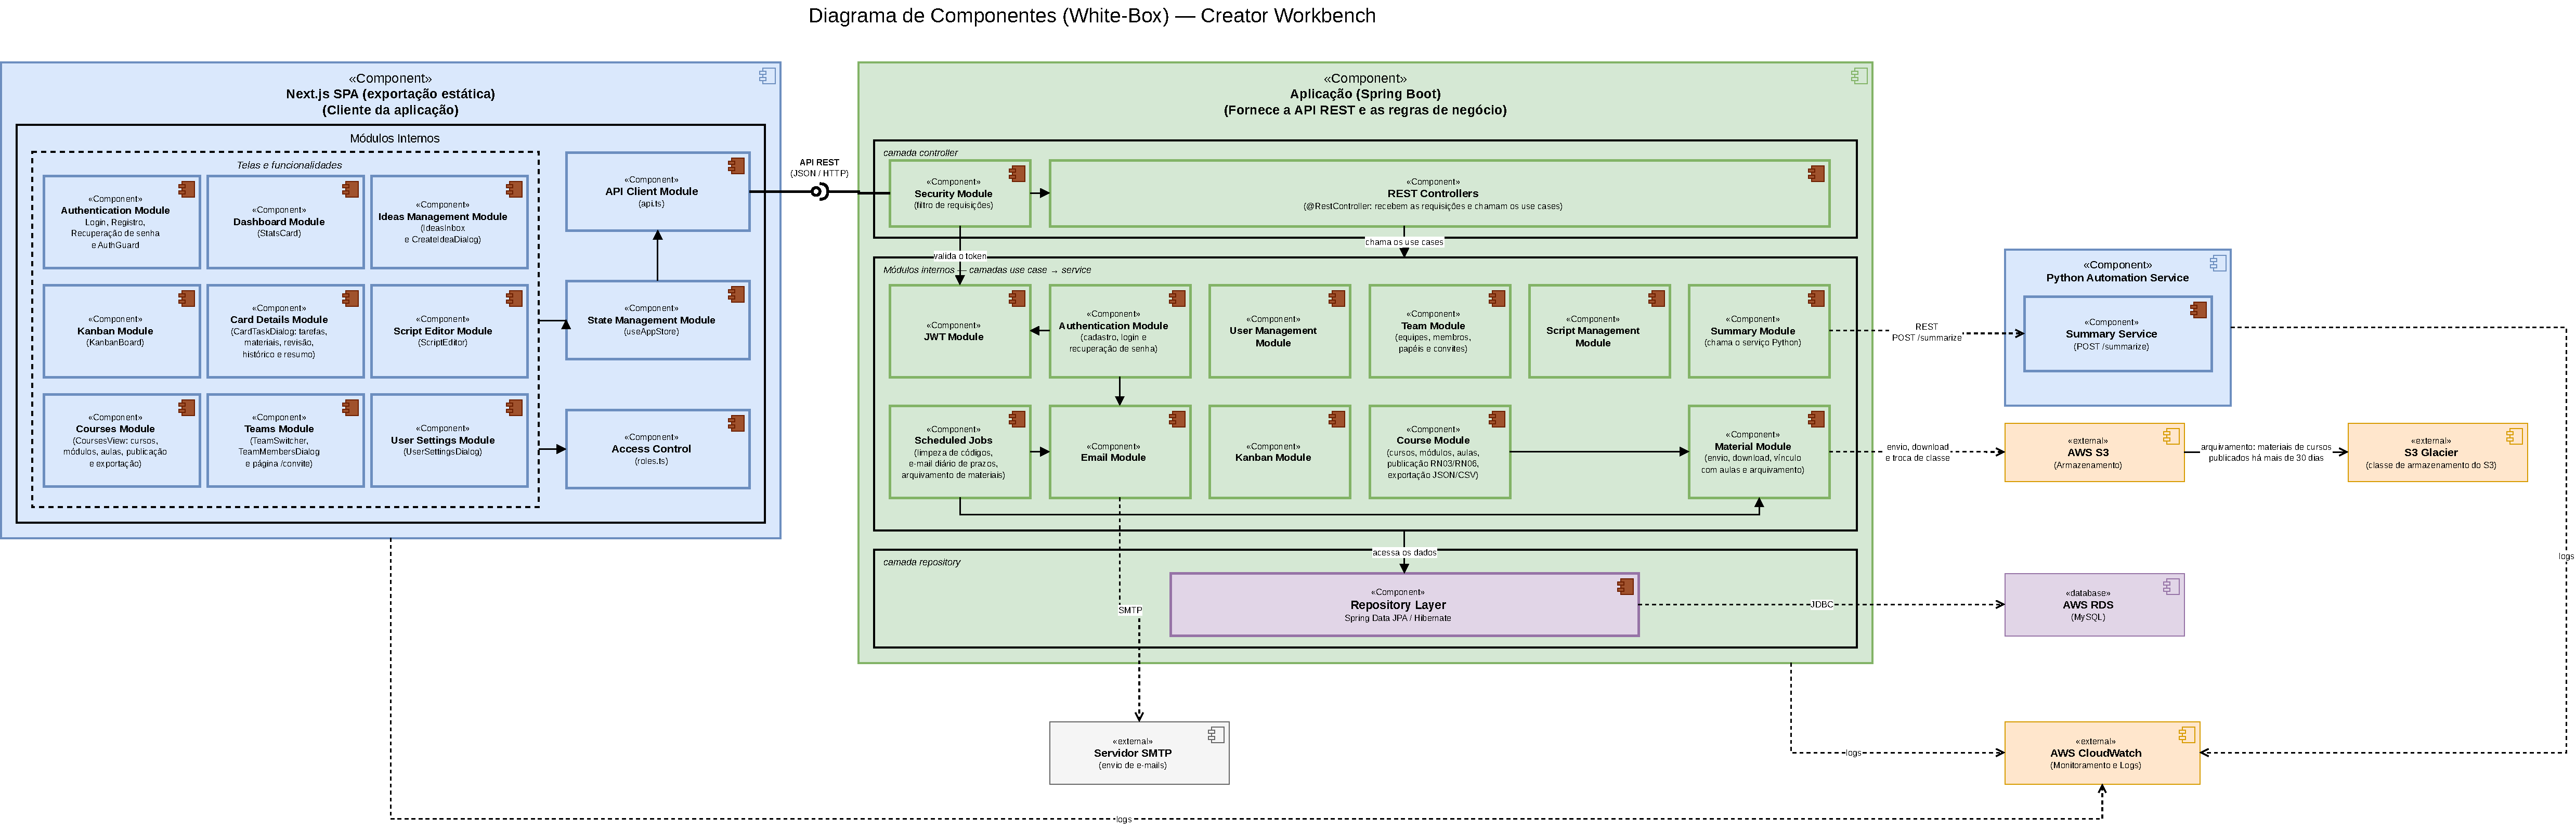
\includegraphics[width=\linewidth,height=14cm,keepaspectratio]{imagens/Diagrama_Componentes.pdf}
        \legend{Fonte: Produzido pelos autores.}
    \end{minipage}}
\end{figure}

\subsection{Diagrama de Implantação}

O diagrama de implantação mostra em que infraestrutura cada parte do sistema roda (Figura~\ref{fig:implantacao}). O usuário acessa o sistema pelo navegador, no computador ou no celular, por HTTP. O acesso chega ao Elastic Load Balancing, dentro da VPC da AWS, que o entrega ao contêiner do \textit{front-end}.

O \textit{cluster} Amazon EKS tem três \textit{namespaces}, um para cada contêiner: \textit{front-end} (Nginx servindo o Next.js em exportação estática), \textit{back-end} (Spring Boot) e automação (serviço em Python). O \textit{front-end} encaminha as chamadas para o \textit{back-end}, que por sua vez chama o serviço de automação. Fora do \textit{cluster} ficam os serviços de apoio: o Amazon RDS (banco de dados MySQL), o Amazon S3 (arquivos e mídias), cujos materiais de cursos publicados há mais de 30 dias passam para a classe S3 Glacier, o Amazon ECR (imagens Docker), o Amazon CloudWatch (\textit{logs}, métricas e alarmes) e o servidor SMTP, usado pelo \textit{back-end} para os e-mails de cadastro, convites e alertas de prazo.

\begin{figure}[p]
    \centering
    \rotatebox{90}{%
    \begin{minipage}{0.95\textheight}
        \centering
        \caption{Diagrama de Implantação - Creator Workbench}
        \label{fig:implantacao}
        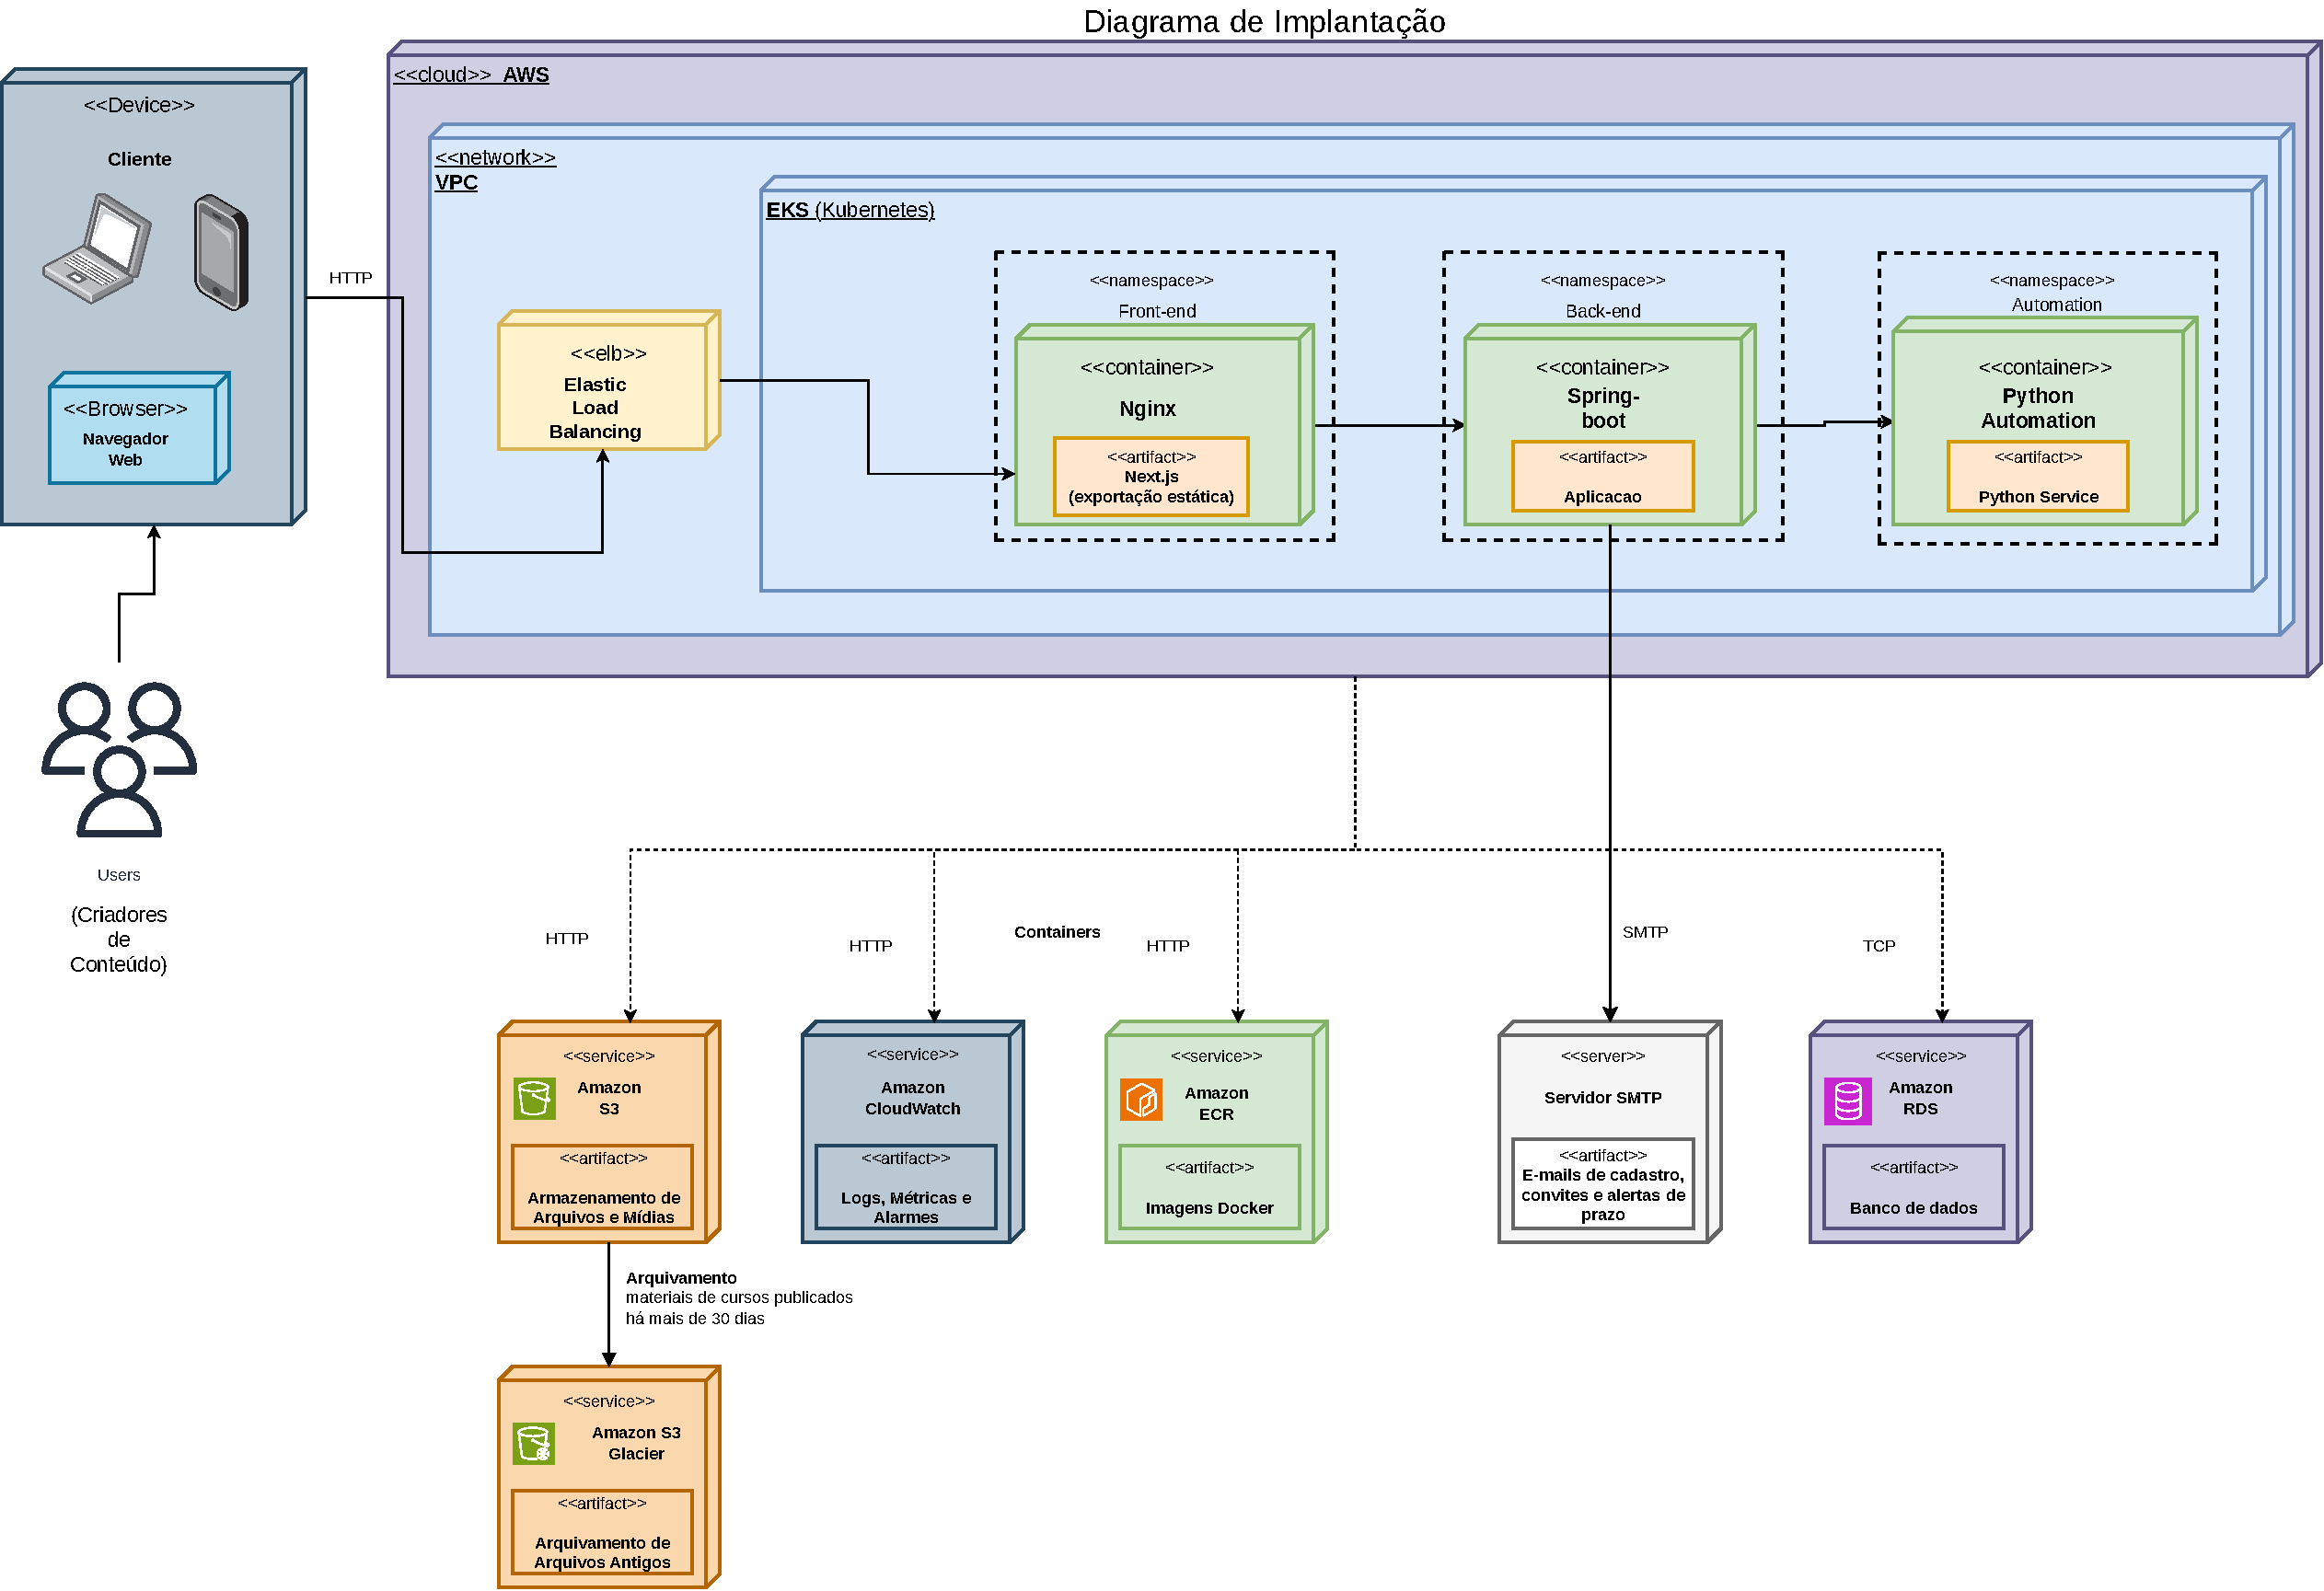
\includegraphics[width=\linewidth,height=14cm,keepaspectratio]{imagens/Diagrama_Implantacao.pdf}
        \legend{Fonte: Produzido pelos autores.}
    \end{minipage}}
\end{figure}

\subsection{Integração com o Serviço de Automação}

O requisito RF08 usa um serviço de automação escrito em Python, que roda em um contêiner próprio, para gerar o resumo do projeto. O resumo exige um roteiro com pelo menos 100 palavras. Com menos que isso, o \textit{back-end} recusa o pedido antes de chamar o serviço e informa que não há dados suficientes. O último resumo gerado fica salvo no projeto, com a data de geração, e pode ser gerado de novo depois de mudanças no roteiro.

O contrato dessa comunicação, ou seja, o que cada lado envia e recebe, é o seguinte:

\begin{itemize}
    \item \textbf{Mecanismo:} chamada REST direta, por HTTP, do \textit{back-end} para o serviço de automação em Python. Os dois rodam no mesmo \textit{cluster}, e o serviço de automação não fica exposto à internet.
    \item \textbf{Tipo de chamada:} síncrona, com limite de 30 segundos.
    \item \textbf{\textit{Endpoint}:} \verb|POST /summarize| no serviço interno de automação.
    \item \textbf{Dados enviados:} um JSON com o texto do roteiro, sem formatação.
    \item \textbf{Dados recebidos:} um JSON com o texto do resumo.
    \item \textbf{Em caso de falha:} se o serviço não responder em 30 segundos ou devolver erro, a API responde com o código 503 e a mensagem ``Não foi possível gerar o resumo agora. Tente novamente.''. O último resumo salvo continua no projeto, e o usuário vê a mensagem na tela.
\end{itemize}

Exemplo dos dados enviados e recebidos:

\begin{small}
\begin{verbatim}
Pedido:   { "text": "<texto do roteiro, sem formatação>" }
Resposta: { "summary": "<texto do resumo>" }
\end{verbatim}
\end{small}

\section{Tecnologias}

As tecnologias foram escolhidas para atender aos requisitos do projeto e à experiência da equipe.

\subsection{Front-end}

O \textit{front-end} é uma \textit{Single Page Application} (SPA) feita com Next.js e React, exportada como arquivos estáticos. Ele usa o \textit{fetch} nativo do navegador para chamar os \textit{endpoints} da API REST e o Zustand para guardar o estado global (equipe ativa, quadro, ideias e cursos).

\begin{table}[H]
\centering
\caption{Tecnologias de \textit{Front-end}}
\label{tab:frontend}
\begin{tabular}{|l|l|p{7cm}|}
\hline
\textbf{Tecnologia} & \textbf{Versão} & \textbf{Finalidade} \\
\hline
Next.js e React (TypeScript) & 16 e 19 & Aplicação de página única, exportada como arquivos estáticos \\
\hline
Tailwind CSS e shadcn/ui & 4 & Estilo e componentes da interface, com tema claro e escuro \\
\hline
Zustand & 5 & Estado global da aplicação \\
\hline
TipTap & - & Editor de texto rico do Estúdio de Escrita \\
\hline
\textit{fetch} nativo & - & Chamadas HTTP para a API \\
\hline
\end{tabular}
\end{table}

\subsection{Back-end}

A API REST segue o nível 2 do Richardson Maturity Model: recursos com nomes claros, verbos HTTP corretos e respostas padronizadas com códigos de status HTTP.

\begin{table}[H]
\centering
\caption{Tecnologias de \textit{Back-end}}
\label{tab:backend}
\begin{tabular}{|l|l|p{7cm}|}
\hline
\textbf{Tecnologia} & \textbf{Versão} & \textbf{Finalidade} \\
\hline
Java e Spring Boot & 21 e 4 & API REST, injeção de dependências e validação \\
\hline
Spring Security e JWT & - & Autenticação e proteção das rotas \\
\hline
Spring Data JPA e Flyway & - & Acesso ao banco e versionamento das tabelas \\
\hline
Spring Mail & - & Envio de códigos, convites e alertas por e-mail \\
\hline
Python & - & Serviço de automação que gera os resumos \\
\hline
Swagger (springdoc) & - & Documentação automática da API (RNF08) \\
\hline
JUnit 5 e Mockito & 5 & Testes unitários (RNF07) \\
\hline
\end{tabular}
\end{table}

\subsection{Banco de Dados}

O banco é modelado e normalizado até a Terceira Forma Normal (3FN), conforme o RNF06, para evitar dados repetidos e garantir a integridade das ligações entre as tabelas. Cada entidade usa um identificador numérico sequencial (\textit{Long}) como chave primária. Os conteúdos (ideias e projetos, roteiros, materiais, cursos, módulos e aulas) têm também um UUID, que serve como identificador público para as automações (RN05).

\begin{table}[H]
\centering
\caption{Tecnologia de Banco de Dados}
\label{tab:bd}
\begin{tabular}{|l|l|}
\hline
\textbf{Tecnologia} & \textbf{Finalidade} \\
\hline
MySQL 8 (Amazon RDS) & Banco de dados relacional principal, normalizado até a 3FN \\
\hline
\end{tabular}
\end{table}

\subsection{Infraestrutura}

A infraestrutura reúne os serviços de nuvem e as ferramentas que fazem o sistema funcionar e ser publicado.

\subsubsection{Amazon Web Services (AWS)}

O sistema roda na AWS, dentro de uma VPC. A Tabela~\ref{tab:aws} mostra os serviços usados e para que cada um serve.

\begin{table}[H]
\centering
\caption{Serviços AWS utilizados}
\label{tab:aws}
\begin{tabular}{|l|p{9cm}|}
\hline
\textbf{Serviço} & \textbf{Finalidade} \\
\hline
Amazon EKS & Orquestração dos contêineres (Kubernetes) \\
\hline
Amazon ECR & Registro das imagens dos contêineres \\
\hline
Elastic Load Balancer & Entrada do acesso dos usuários, que entrega o tráfego ao \textit{front-end} \\
\hline
Amazon RDS (MySQL) & Banco de dados relacional gerenciado, acessível apenas de dentro da VPC \\
\hline
Amazon S3 e S3 Glacier & Materiais dos projetos e arquivamento dos materiais de cursos publicados há mais de 30 dias (RN04) \\
\hline
Amazon CloudWatch Logs & \textit{Logs} dos contêineres (RNF10) \\
\hline
\end{tabular}
\end{table}

\subsubsection{Docker e Contêineres}

O sistema roda em três contêineres Docker: o \textit{front-end} (Nginx servindo os arquivos estáticos do Next.js), o \textit{back-end} (Spring Boot) e o serviço de automação em Python. As imagens ficam no Amazon ECR e o Amazon EKS orquestra a execução (RNF09). Os contêineres deixam o ambiente de execução igual entre o desenvolvimento e a produção.

\subsubsection{Integração Contínua (CI)}

O GitHub Actions executa os testes automaticamente a cada envio de código. Os relatórios de cobertura ficam publicados no ambiente de demonstração.

\section{Testes e Manutenibilidade}

Os testes e a análise de código ajudam a garantir que o sistema funcione como o esperado e continue fácil de manter.

\subsection{Plano de Testes}

O plano de testes segue uma abordagem em pirâmide. Na base ficam os testes unitários, que são mais baratos de manter, e acima deles os testes de integração e de componentes. O \textit{back-end} tem testes unitários para os casos de uso e serviços, escritos com JUnit 5 e Mockito. O \textit{front-end} tem testes de componentes, da \textit{store} e das funções de acesso à API, escritos com Jest e Testing Library. Os cenários de teste (CT01 a CT17) estão ligados às histórias de usuário na Tabela~\ref{tab:rastreabilidade}.

\subsection{Análise Estática}

O SonarQube analisa o código a cada entrega e aplica um indicador de qualidade (\textit{quality gate}) ao \textit{back-end}. Os testes rodam automaticamente no GitHub Actions.

\subsection{Cobertura e Resultados dos Testes}

A cobertura dos testes do \textit{back-end} é medida pelo JaCoCo. Na versão final, a cobertura de linhas é superior a 80\%, acima da meta de 70\% definida no RNF07. A Tabela~\ref{tab:cobertura} mostra a cobertura por pacote.

\begin{table}[H]
\centering
\caption{Cobertura de testes por pacote (JaCoCo)}
\label{tab:cobertura}
\begin{tabular}{|l|r|}
\hline
\textbf{Pacote} & \textbf{Cobertura de linhas} \\
\hline
\textit{controller} & [PREENCHER]\% \\
\hline
\textit{usecase} & [PREENCHER]\% \\
\hline
\textit{service} & [PREENCHER]\% \\
\hline
\textit{config} & [PREENCHER]\% \\
\hline
\textit{entity} & [PREENCHER]\% \\
\hline
\textbf{Total} & \textbf{[PREENCHER]\%} \\
\hline
\end{tabular}
\end{table}

O número final de testes e o resultado da execução estão no relatório de testes da entrega: [PREENCHER: número de testes e resultado].

\section{Segurança, Privacidade e Legislação}

A segurança dos dados dos usuários é parte do projeto desde o início. Esta seção mostra as medidas técnicas e como o sistema atende à lei de proteção de dados.

\subsection{Critérios de Segurança e Privacidade}

O sistema tem segurança em várias camadas:

\textbf{Autenticação e Autorização:} o acesso é controlado por funções (RBAC) em cada equipe, com três papéis: Administrador, Criador e Revisor (RF02). O \textit{back-end} confere o papel em toda requisição. Se alguém tentar uma ação sem permissão, a API responde com o código 403. Os \textit{tokens} JWT são assinados e valem 24 horas (RNF03).

\textbf{Proteção de Dados:} as senhas são guardadas somente como \textit{hash} gerado pelo algoritmo BCrypt (RNF01) e nunca aparecem nas respostas da API.

\textbf{Códigos e Convites:} os códigos enviados por e-mail valem 10 minutos e aceitam até 5 tentativas. Os convites valem 7 dias e só podem ser aceitos pela conta com o mesmo e-mail.

\textbf{Rede:} o banco de dados só pode ser acessado de dentro da VPC, e o serviço de automação não fica exposto à internet.

\subsection{Observância à Legislação}

O sistema é desenvolvido de acordo com a Lei Geral de Proteção de Dados Pessoais (LGPD, Lei n\textsuperscript{o} 13.709/2018), que regula o tratamento de dados pessoais no Brasil. As principais medidas são: coleta mínima de dados (apenas nome e e-mail no cadastro), senhas protegidas com BCrypt e possibilidade de o próprio usuário excluir a conta. Os dados pessoais não são compartilhados com terceiros sem o consentimento do titular.

\section{Modelo de Banco de Dados}

O modelo de banco de dados organiza as informações do sistema. Esta seção apresenta o MER, o DER, o diagrama de classes e o dicionário de dados.

\subsection{Modelo Entidade-Relacionamento (MER)}

O modelo é construído em torno das entidades principais do sistema: Usuário, Equipe, Membro da equipe (que guarda o papel de cada pessoa em cada equipe), Convite, Etiqueta, Coluna, Ideia e Projeto (\textit{card}), Tarefa, Material, Roteiro e suas versões, Revisão, Curso, Módulo e Aula. Cada entidade tem um identificador numérico sequencial como chave primária, e os conteúdos têm também um UUID (RN05).

\subsection{Figura do Modelo Entidade-Relacionamento}

A figura a seguir apresenta o MER do Creator Workbench.

\begin{figure}[H]
    \caption{Modelo Entidade-Relacionamento - Creator Workbench}
    \centering
    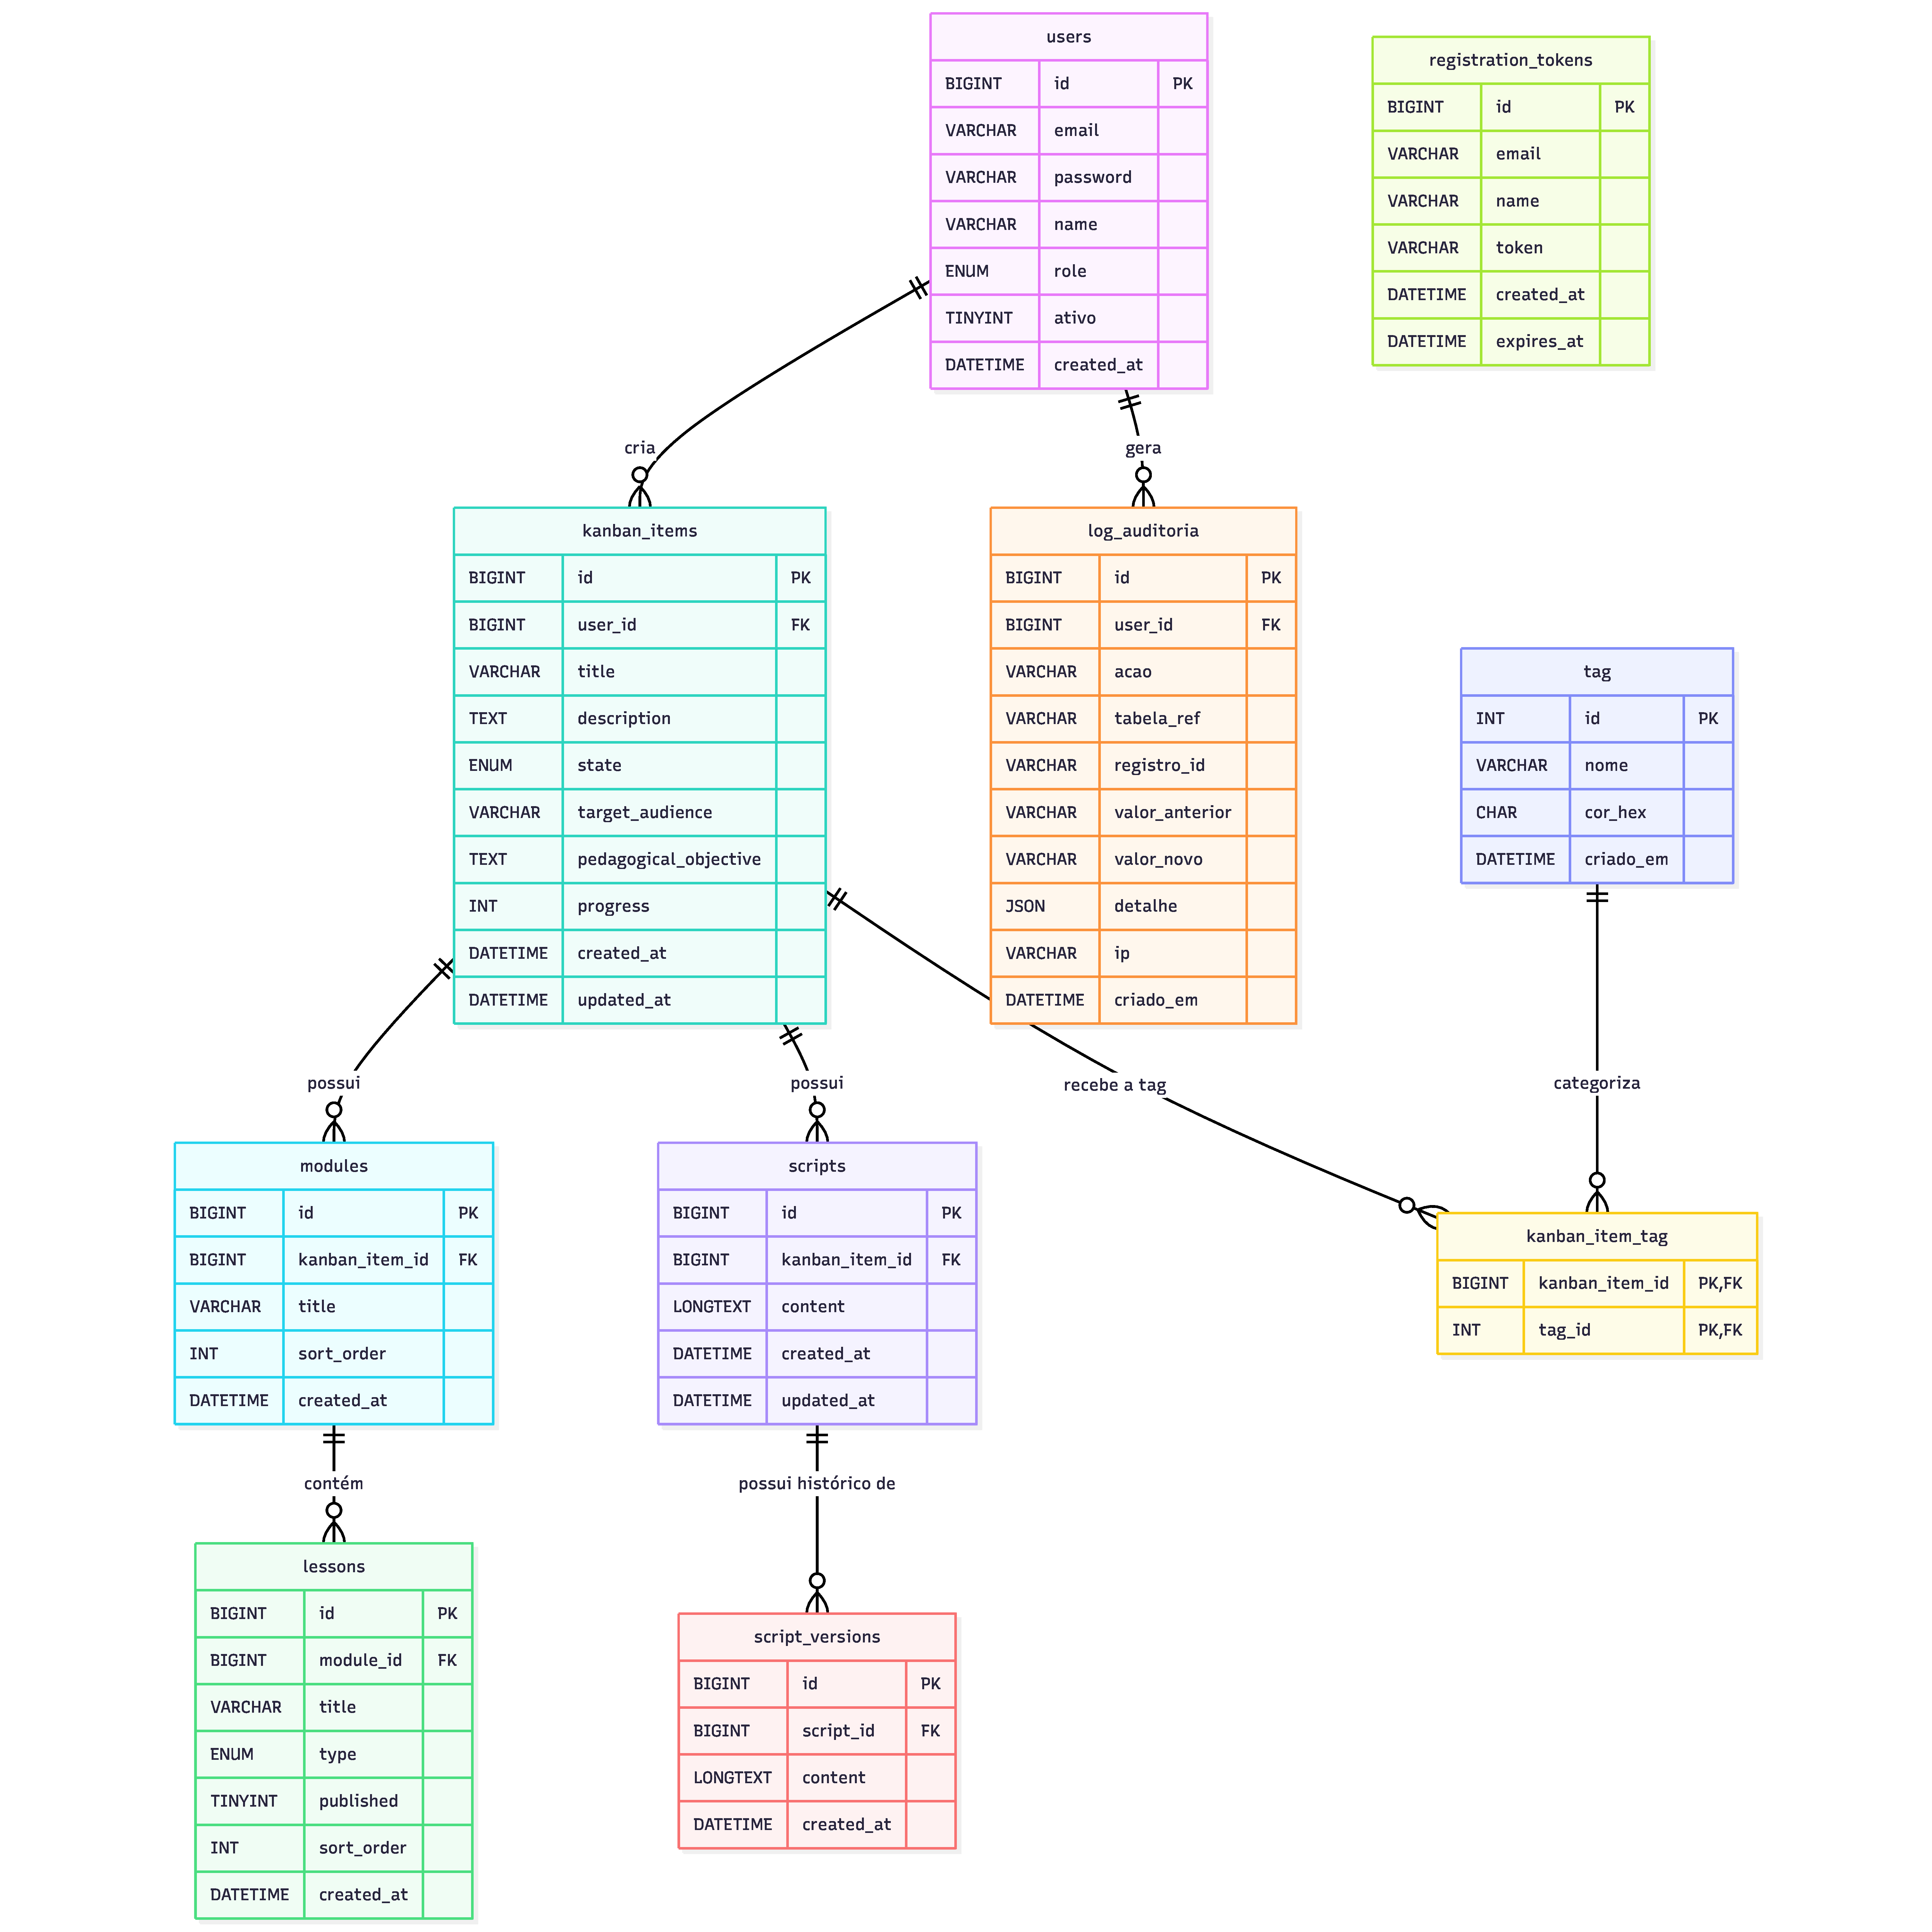
\includegraphics[width=\textwidth]{imagens/der.pdf}
    \label{fig:mer}
    \legend{Fonte: Produzido pelos autores.}
\end{figure}

\subsection{Diagrama Entidade-Relacionamento (DER)}

O DER mostra como o modelo conceitual virou tabelas no banco de dados, com as colunas e as ligações entre elas.

\begin{figure}[H]
    \caption{Diagrama Entidade-Relacionamento - Creator Workbench}
    \centering
    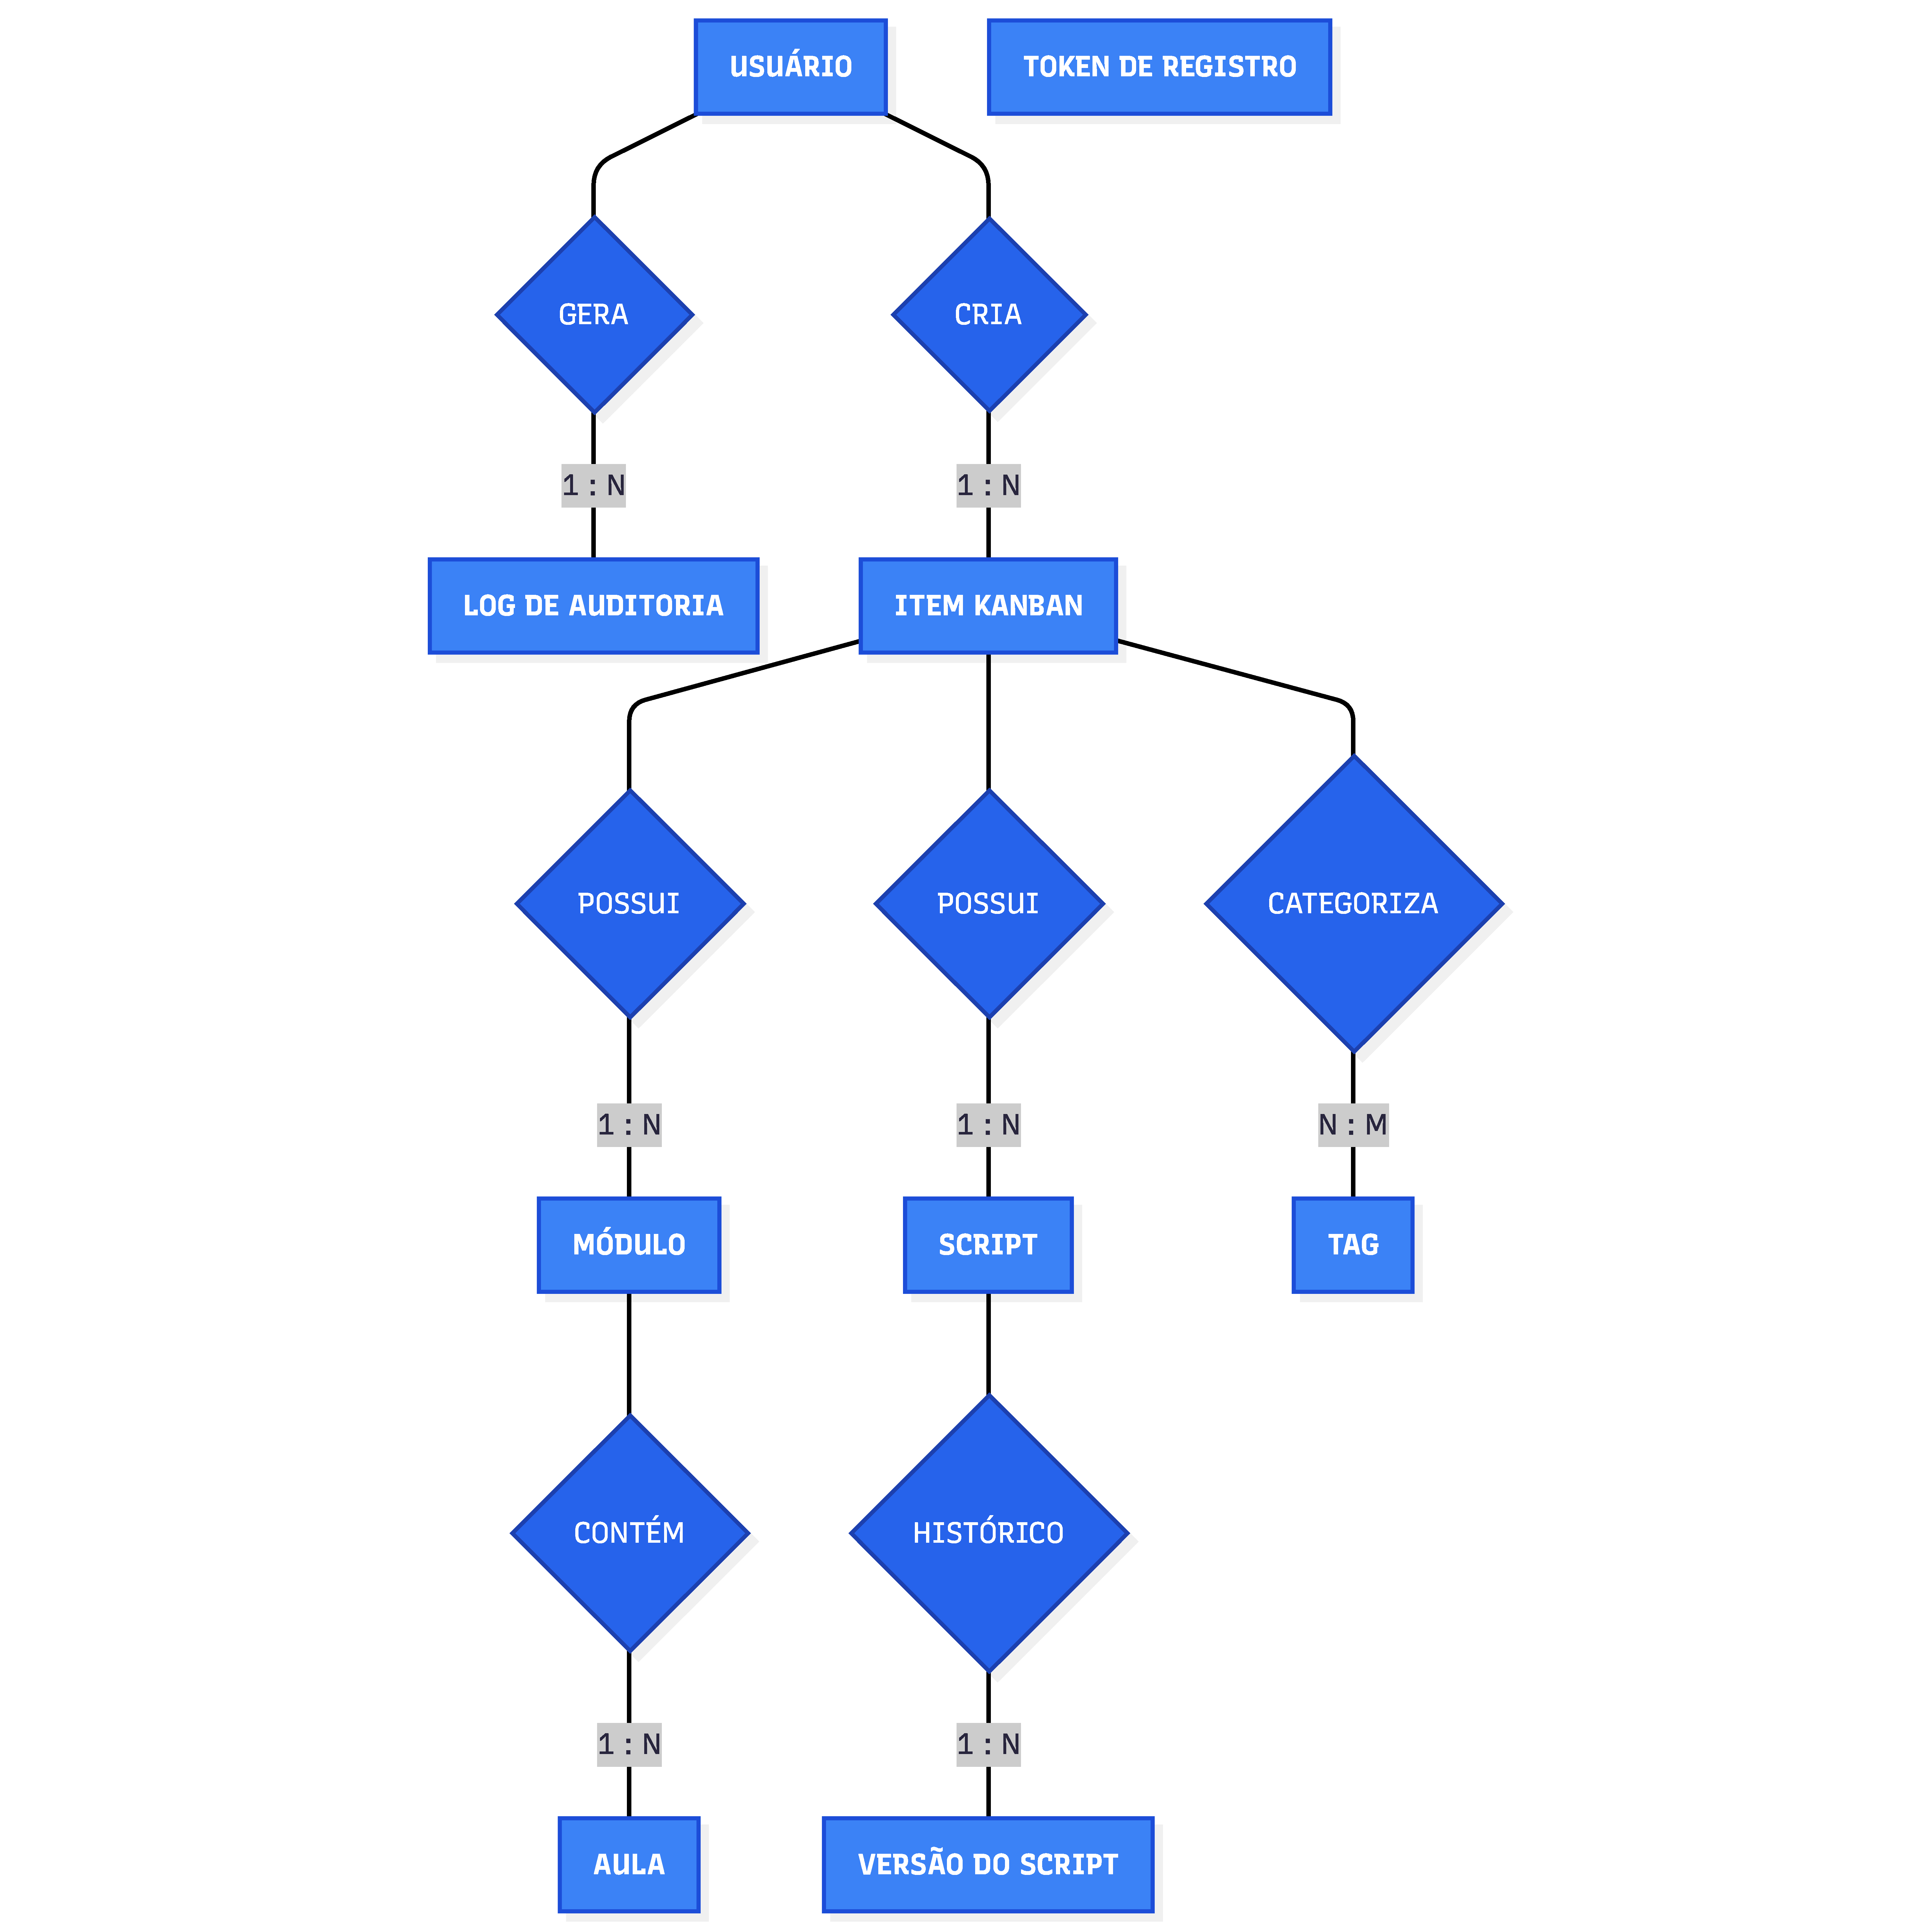
\includegraphics[width=\textwidth]{imagens/mer.pdf}
    \label{fig:der}
    \legend{Fonte: Produzido pelos autores.}
\end{figure}

\subsection{Diagrama de Classes}

O diagrama de classes mostra como as entidades do sistema são representadas no código do \textit{back-end} (Figura~\ref{fig:classes}). São 22 classes e 9 enumerações, agrupadas por módulo: usuários e equipes; quadro, ideias e projetos; materiais e roteiro; cursos; e códigos de verificação.

Cada classe mostra seus atributos e métodos, com a visibilidade de cada um. As ligações com losango preenchido indicam composição, em que a parte não existe sem o todo: uma tarefa, por exemplo, só existe dentro de um projeto. As demais ligações são associações simples, com as multiplicidades em cada ponta. Os atributos marcados com barra (/), como o progresso e a situação da revisão do projeto, são derivados: o sistema os calcula e eles não são gravados no banco. A classe \textit{LessonMaterial} é uma classe de associação, que liga uma aula a um material.

\begin{figure}[p]
    \centering
    \rotatebox{90}{%
    \begin{minipage}{0.95\textheight}
        \centering
        \caption{Diagrama de Classes - Creator Workbench}
        \label{fig:classes}
        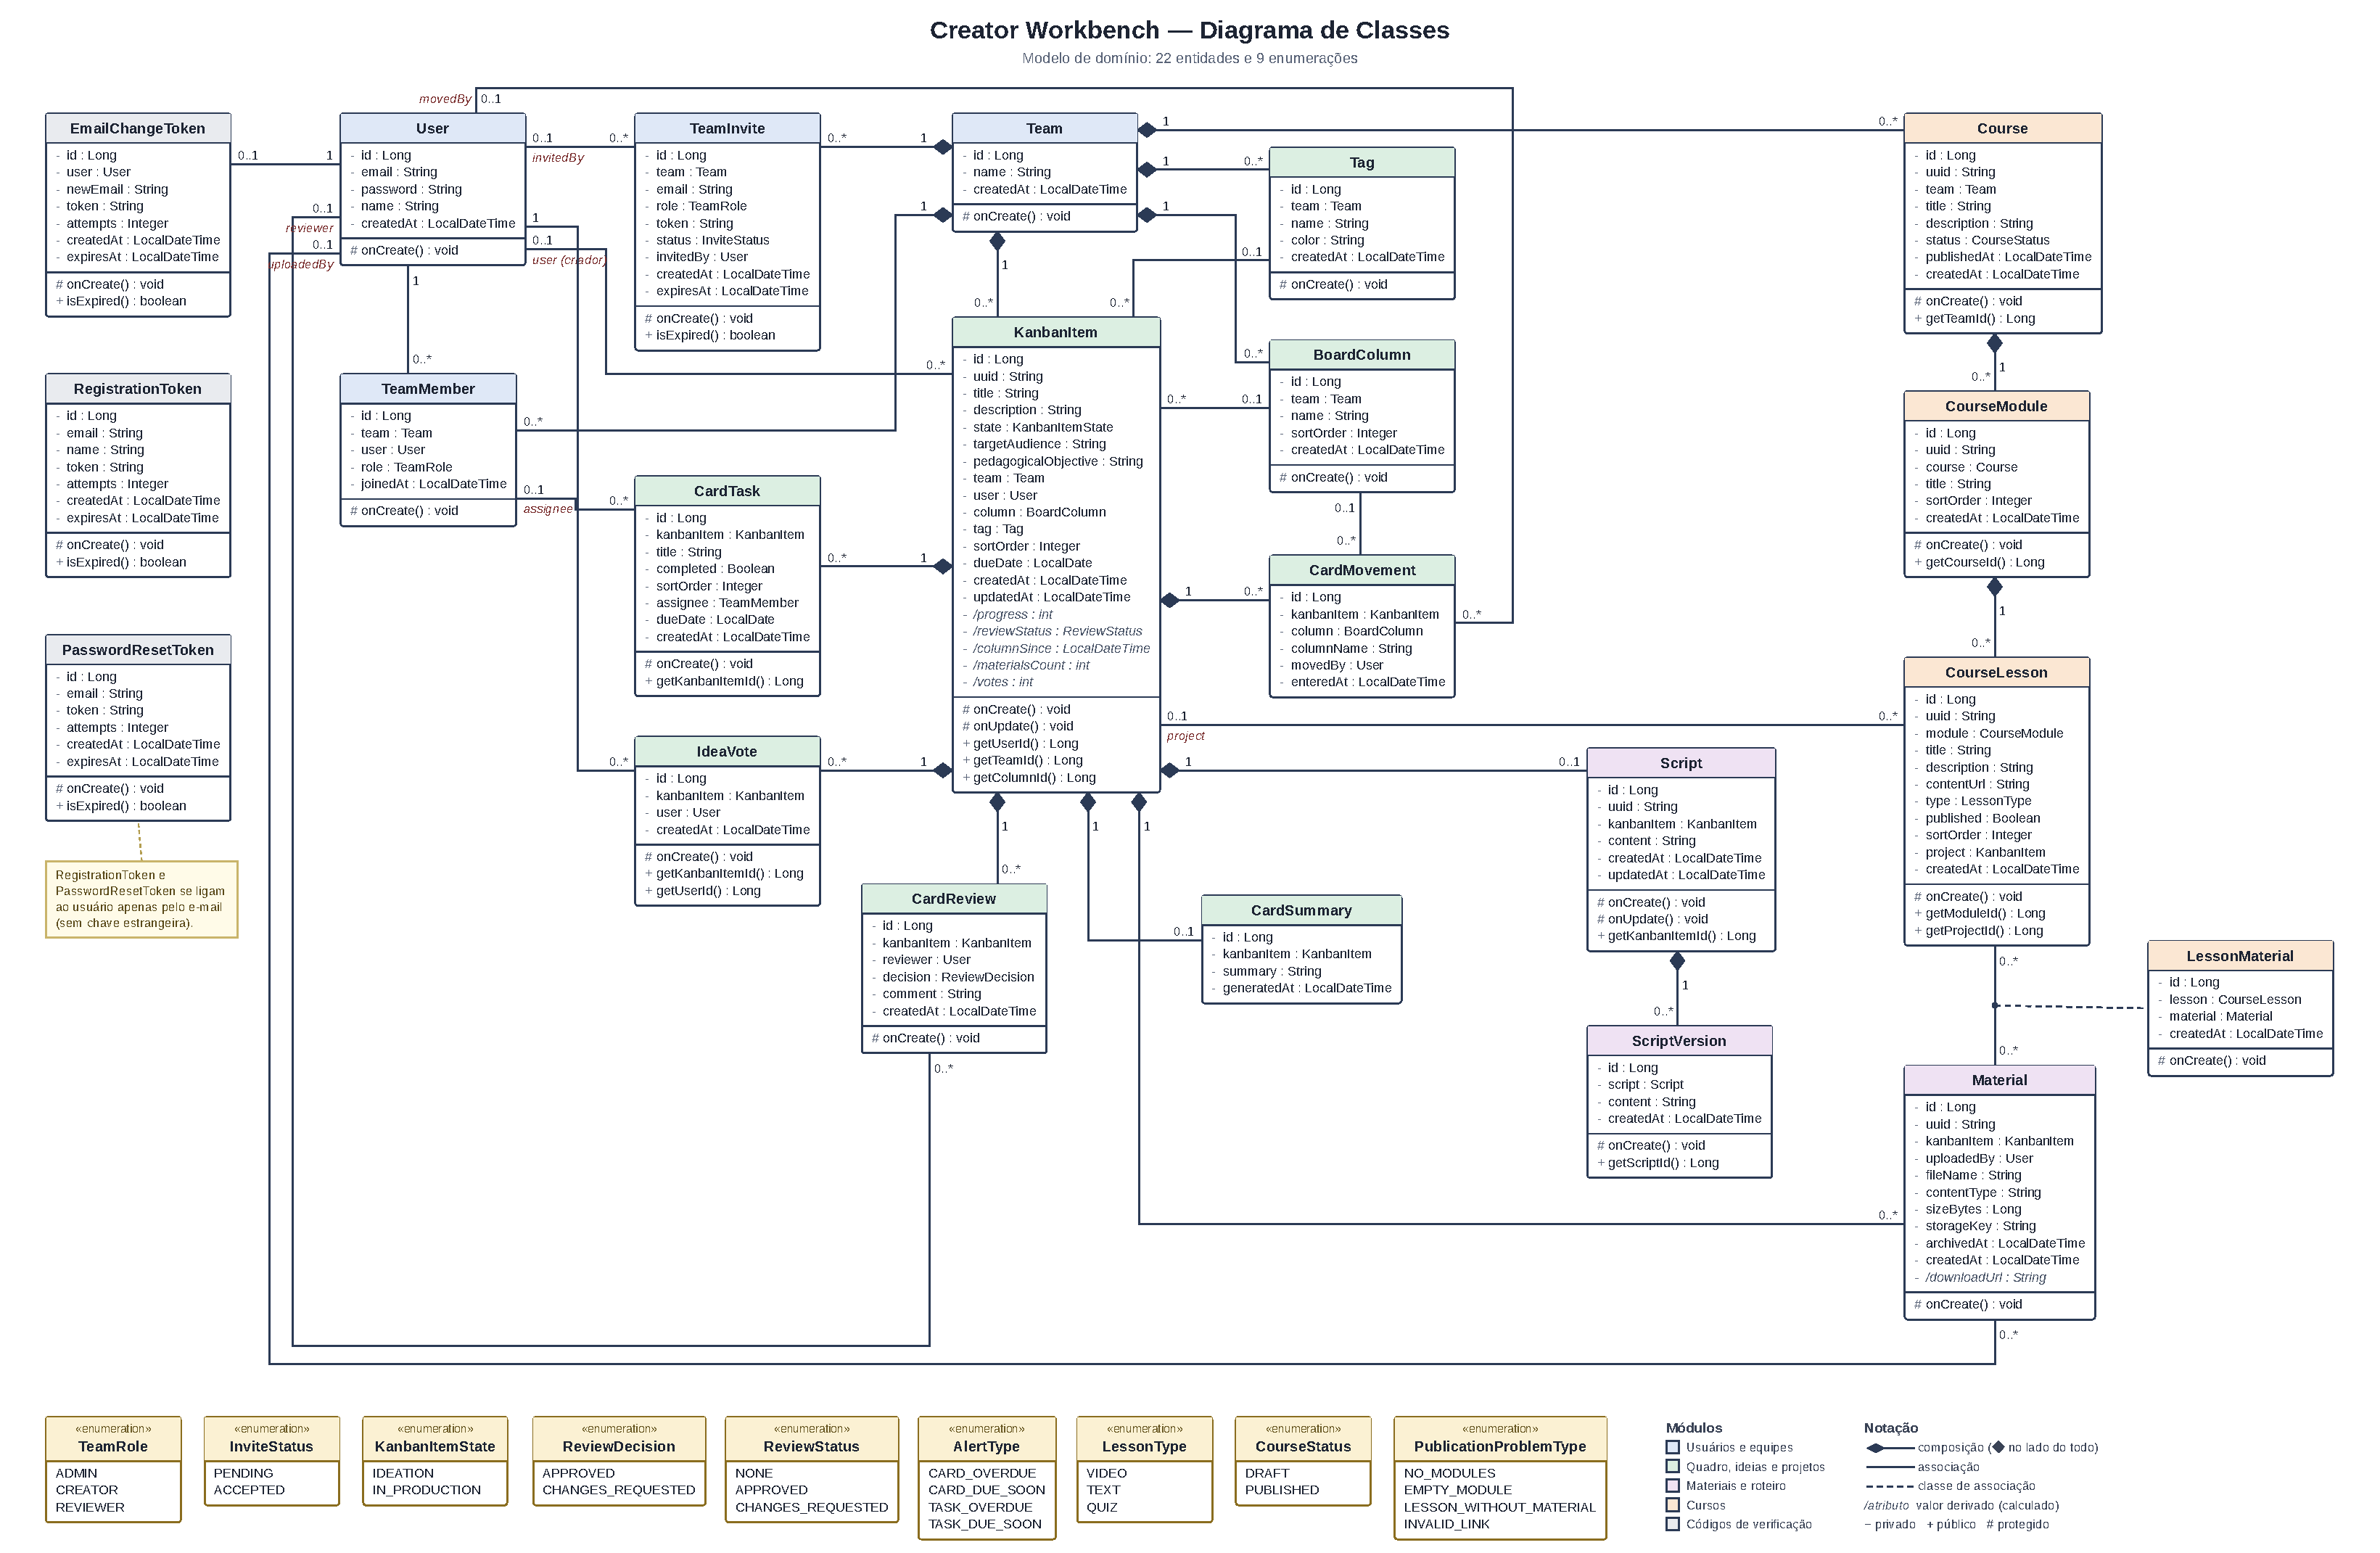
\includegraphics[width=\linewidth,height=14cm,keepaspectratio]{imagens/diagrama-de-classes.pdf}
        \legend{Fonte: Produzido pelos autores.}
    \end{minipage}}
\end{figure}

\subsection{Dicionário de Dados}

O dicionário de dados descreve cada campo das principais tabelas: nome, tipo, restrições e significado. Os nomes e os tipos abaixo devem ser conferidos com as migrações Flyway do projeto.

\begin{table}[H]
\centering
\caption{Dicionário de Dados: Entidade Usuário}
\label{tab:dd-usuario}
\begin{tabular}{|l|l|l|p{5cm}|}
\hline
\textbf{Atributo} & \textbf{Tipo} & \textbf{Restrição} & \textbf{Descrição} \\
\hline
id & BIGINT & PK, NOT NULL & Identificador único do usuário \\
\hline
nome & VARCHAR(150) & NOT NULL & Nome completo do usuário \\
\hline
email & VARCHAR(255) & UNIQUE, NOT NULL & E-mail de login e de notificações \\
\hline
senha\_hash & VARCHAR(255) & NOT NULL & \textit{Hash} BCrypt da senha \\
\hline
created\_at & TIMESTAMP & NOT NULL & Data e hora de criação do registro \\
\hline
\end{tabular}
\end{table}

\begin{table}[H]
\centering
\caption{Dicionário de Dados: Entidade Membro da Equipe}
\label{tab:dd-membro}
\begin{tabular}{|l|l|l|p{5cm}|}
\hline
\textbf{Atributo} & \textbf{Tipo} & \textbf{Restrição} & \textbf{Descrição} \\
\hline
id & BIGINT & PK, NOT NULL & Identificador único do membro \\
\hline
usuario\_id & BIGINT & FK, NOT NULL & Referência ao usuário \\
\hline
equipe\_id & BIGINT & FK, NOT NULL & Referência à equipe \\
\hline
papel & ENUM & NOT NULL & Papel na equipe: ADMINISTRADOR, CRIADOR, REVISOR \\
\hline
\end{tabular}
\end{table}

\begin{table}[H]
\centering
\small
\caption{Dicionário de Dados: Entidade Projeto}
\label{tab:dd-projeto}
\begin{tabular}{|>{\raggedright\arraybackslash}p{3.6cm}|>{\raggedright\arraybackslash}p{2.8cm}|>{\raggedright\arraybackslash}p{3cm}|>{\raggedright\arraybackslash}p{4.8cm}|}
\hline
\textbf{Atributo} & \textbf{Tipo} & \textbf{Restrição} & \textbf{Descrição} \\
\hline
id & BIGINT & PK, NOT NULL & Identificador único do projeto \\
\hline
uuid & CHAR(36) & UNIQUE, NOT NULL & Identificador público para automações (RN05) \\
\hline
titulo & VARCHAR(255) & NOT NULL & Título do conteúdo em produção \\
\hline
publico\_alvo & TEXT & NOT NULL & Público-alvo (obrigatório para converter, RN01) \\
\hline
objetivo\_pedagogico & TEXT & NOT NULL & Objetivo pedagógico (obrigatório, RN01) \\
\hline
coluna\_id & BIGINT & FK, NOT NULL & Coluna do quadro em que o projeto está \\
\hline
prazo & DATE & NULL & Data de entrega do projeto \\
\hline
equipe\_id & BIGINT & FK, NOT NULL & Equipe dona do projeto \\
\hline
\end{tabular}
\par\small Fonte: Produzido pelos autores.
\end{table}

\section{Duração / Cronograma}

O cronograma mostra quanto tempo o projeto leva e o que é entregue em cada etapa.

\subsection{Análise da Duração do Projeto}

O projeto é organizado em 8 Sprints quinzenais, totalizando aproximadamente 16 semanas de desenvolvimento. A duração foi definida pela complexidade do escopo do MVP, e não pelo calendário do semestre, conforme a orientação metodológica. A Tabela~\ref{tab:cronograma} mostra o planejamento inicial, e a Tabela~\ref{tab:sprints}, no capítulo de Gestão do Projeto, mostra o que foi de fato entregue em cada Sprint.

\begin{table}[H]
\centering
\caption{Cronograma de Sprints (planejamento inicial)}
\label{tab:cronograma}
\begin{tabular}{|l|l|p{8cm}|}
\hline
\textbf{Sprint} & \textbf{Duração} & \textbf{Entregas Previstas} \\
\hline
Sprint 1 & Semanas 1--2 & \textit{Setup} da infraestrutura (AWS, Docker, CI), modelagem do banco de dados \\
\hline
Sprint 2 & Semanas 3--4 & Módulo de autenticação e equipes (RF01, RF02, RNF01, RNF03) \\
\hline
Sprint 3 & Semanas 5--6 & Módulo de Gestão de Ideias, Caixa de Entrada (RF03, RF04) \\
\hline
Sprint 4 & Semanas 7--8 & Módulo de Produção, \textit{Kanban} e tarefas (RF05) \\
\hline
Sprint 5 & Semanas 9--10 & Materiais e Estúdio de Escrita (RF06, RF07) \\
\hline
Sprint 6 & Semanas 11--12 & Módulo de Automação, resumo e alertas (RF08, RF09) \\
\hline
Sprint 7 & Semanas 13--14 & Módulo Curricular, Cursos, Módulos, Aulas, exportação (RF10, RF11) \\
\hline
Sprint 8 & Semanas 15--16 & Testes, ajustes de performance, documentação final \\
\hline
\end{tabular}
\end{table}

\chapter{Viabilidade Financeira}

Este capítulo analisa se o Creator Workbench pode se manter com o dinheiro que arrecada. Primeiro apresenta os custos, depois a receita dos planos de assinatura e, por fim, três cenários de projeção para os primeiros 12 meses.

\section{Custos}

Os custos do projeto são divididos em duas categorias: desenvolvimento (a mão de obra da equipe acadêmica, considerada como custo de oportunidade) e infraestrutura operacional.

A infraestrutura entregue usa o Amazon EKS ligado 24 horas por dia, e por isso o custo é maior que o de um servidor simples. A tabela abaixo mostra a estimativa mensal, com valores de referência sob demanda, na região us-east-1, para 730 horas por mês \cite{aws2026}. Os valores em reais foram convertidos pela cotação de R\$ 5,3420 por dólar, a mesma usada na Tabela~\ref{tab:comparativo}.

\begin{table}[H]
\centering
\small
\caption{Infraestrutura Mensal Estimada}
\label{tab:infra}
\begin{tabular}{|p{8cm}|r|r|}
\hline
\textbf{Item} & \textbf{Dólar} & \textbf{Real} \\
\hline
Amazon EKS (plano de controle do \textit{cluster}) & US\$ 73,00 & R\$ 389,97 \\
\hline
2 nós EC2 t3.medium do \textit{cluster} & US\$ 60,74 & R\$ 324,47 \\
\hline
Elastic Load Balancer (Application Load Balancer) & US\$ 22,00 & R\$ 117,52 \\
\hline
Amazon RDS MySQL db.t3.micro com 20 GB & US\$ 14,71 & R\$ 78,58 \\
\hline
Discos dos nós (2 x 20 GB EBS gp3) & US\$ 3,20 & R\$ 17,09 \\
\hline
Endereços IPv4 públicos (4) & US\$ 14,60 & R\$ 77,99 \\
\hline
Amazon S3 e S3 Glacier (cerca de 50 GB) & US\$ 2,00 & R\$ 10,68 \\
\hline
Amazon ECR (imagens dos contêineres) & US\$ 0,15 & R\$ 0,80 \\
\hline
Amazon CloudWatch Logs (cerca de 5 GB) & US\$ 3,00 & R\$ 16,03 \\
\hline
Transferência de dados e envio de e-mails & US\$ 4,00 & R\$ 21,37 \\
\hline
Domínio e certificado & - & R\$ 10,00 \\
\hline
\textbf{Total mensal} & \textbf{US\$ 197,40} & \textbf{R\$ 1.064,50} \\
\hline
\end{tabular}
\end{table}

\section{Receitas}

O modelo de monetização proposto é o SaaS (\textit{Software as a Service}), com planos de assinatura mensais. Toda equipe começa no plano Gratuito. O administrador da equipe pode testar uma vez, por 14 dias, o plano Solo, Pro ou Agência, e ao fim do teste a equipe volta ao plano Gratuito. A ativação do plano pago é feita pela administração do sistema, e a integração com um meio de pagamento fica como trabalho futuro.

\begin{table}[H]
\centering
\small
\caption{Planos de Assinatura}
\label{tab:planos}
\begin{tabular}{|>{\raggedright\arraybackslash}p{2cm}|>{\raggedright\arraybackslash}p{3.6cm}|r|>{\raggedright\arraybackslash}p{6cm}|}
\hline
\textbf{Plano} & \textbf{Público} & \textbf{Preço Mensal} & \textbf{Funcionalidades} \\
\hline
Gratuito & Quem quer conhecer o sistema & R\$ 0,00 & 1 usuário, até 3 projetos ativos, 1 curso, até 100 MB de materiais e sem resumo automático \\
\hline
Solo & Professor autônomo & R\$ 49,00 & 1 usuário, até 10 projetos ativos \\
\hline
Pro & Criador profissional & R\$ 99,00 & 1 usuário, projetos ilimitados, automações \\
\hline
Agência & Pequenas equipes & R\$ 249,00 & Até 5 usuários, controle de acesso completo (RBAC) \\
\hline
\end{tabular}
\par\small Fonte: Produzido pelos autores.
\end{table}

Como os planos pagos têm preços diferentes, a receita depende de quantos assinantes escolhem cada um. Por isso, em cada cenário a seguir é mostrado o mix de planos usado no cálculo. As premissas da equipe são:

\begin{itemize}
    \item \textbf{Mix de planos pagos:} 65\% Solo, 28\% Pro e 7\% Agência. O valor médio por assinante pagante é de cerca de R\$ 77,00 (0,65 $\times$ 49 + 0,28 $\times$ 99 + 0,07 $\times$ 249).
    \item \textbf{Conversão:} 4\% dos usuários do plano Gratuito passam a um plano pago, e 20\% das equipes que fazem o teste de 14 dias continuam no plano pago.
    \item \textbf{Custo de infraestrutura:} R\$ 1.064,50 por mês, como na Tabela~\ref{tab:infra}.
\end{itemize}

A receita bruta é a soma dos preços de todas as assinaturas pagas, antes de impostos e de taxas de pagamento. O resultado é a receita bruta menos o custo de infraestrutura, e a margem é o resultado dividido pela receita bruta. Com o custo de R\$ 1.064,50 e o valor médio de R\$ 77,00, a operação se paga a partir de 14 assinantes pagantes. A margem passa de 90\% a partir de 139 assinantes pagantes.

\subsection{Cenário Realista}

Projeção para os primeiros 12 meses depois do lançamento, com crescimento moderado, vindo de indicações e de buscas na internet (SEO). Nesse cenário, a maior parte dos assinantes escolhe o plano Solo, que é o mais barato.

\begin{table}[H]
\centering
\small
\caption{Mix de planos e receita: Cenário Realista}
\label{tab:mix-realista}
\begin{tabular}{|l|p{6.2cm}|r|}
\hline
\textbf{Mês} & \textbf{Mix de planos e cálculo} & \textbf{Receita Bruta} \\
\hline
1 a 3 & 15 assinantes: 10 Solo (R\$ 490,00) + 4 Pro (R\$ 396,00) + 1 Agência (R\$ 249,00) & R\$ 1.135,00 \\
\hline
4 a 6 & 40 assinantes: 26 Solo (R\$ 1.274,00) + 11 Pro (R\$ 1.089,00) + 3 Agência (R\$ 747,00) & R\$ 3.110,00 \\
\hline
7 a 12 & 100 assinantes: 65 Solo (R\$ 3.185,00) + 28 Pro (R\$ 2.772,00) + 7 Agência (R\$ 1.743,00) & R\$ 7.700,00 \\
\hline
\end{tabular}
\end{table}

\begin{table}[H]
\centering
\small
\caption{Projeção Financeira: Cenário Realista}
\label{tab:realista}
\begin{tabular}{|l|r|r|r|r|r|}
\hline
\textbf{Mês} & \textbf{Assinantes} & \textbf{Receita Bruta} & \textbf{Custo Infra} & \textbf{Resultado} & \textbf{Margem} \\
\hline
1 a 3  & 15  & R\$ 1.135,00 & R\$ 1.064,50 & R\$ 70,50    & 6,2\% \\
\hline
4 a 6  & 40  & R\$ 3.110,00 & R\$ 1.064,50 & R\$ 2.045,50 & 65,8\% \\
\hline
7 a 12 & 100 & R\$ 7.700,00 & R\$ 1.064,50 & R\$ 6.635,50 & 86,2\% \\
\hline
\end{tabular}
\end{table}

Pela conversão de 4\%, esses números de assinantes equivalem a cerca de 375, 1.000 e 2.500 usuários no plano Gratuito. Nos primeiros meses o resultado é pequeno, e a operação só cobre o custo com folga a partir do quarto mês.

\subsection{Cenário Otimista}

Adoção mais rápida, com parcerias com produtoras de cursos e lançamento em comunidades de criadores. A meta é chegar a 300 assinantes em 12 meses, com o mesmo mix de planos do cenário realista: 195 Solo (R\$ 9.555,00) + 84 Pro (R\$ 8.316,00) + 21 Agência (R\$ 5.229,00), o que dá uma receita bruta de R\$ 23.100,00 por mês. Com o custo de R\$ 1.064,50, o resultado é de R\$ 22.035,50 e a margem é de 95,4\%. Essa margem continua acima de 90\% enquanto o custo de infraestrutura ficar abaixo de cerca de R\$ 2.310,00 por mês, o que permite um \textit{cluster} maior para esse volume. Pela conversão de 4\%, esse cenário equivale a cerca de 7.500 usuários no plano Gratuito.

\subsection{Cenário Pessimista}

Adoção lenta, com 30 assinantes ao final do primeiro ano: 22 Solo (R\$ 1.078,00) + 7 Pro (R\$ 693,00) + 1 Agência (R\$ 249,00), o que dá uma receita bruta de R\$ 2.020,00 por mês. Com o custo de R\$ 1.064,50, o resultado é de R\$ 955,50 e a margem é de 47,3\%. Esse valor cobre o custo de infraestrutura e mantém o produto no ar, mas não traz retorno relevante sobre o investimento de desenvolvimento. Nesse cenário, a estratégia para melhorar a situação é divulgar mais o plano Gratuito e o teste de 14 dias, para aumentar o número de usuários e validar o produto.